\documentclass[12pt, twoside]{article}
\usepackage[letterpaper, margin=1in, headsep=0.2in]{geometry}
\setlength{\headheight}{0.6in}
%\usepackage[english]{babel}
\usepackage[utf8]{inputenc}
\usepackage{microtype}
\usepackage{amsmath}
\usepackage{amssymb}
%\usepackage{amsfonts}
\usepackage{siunitx} %units in math. eg 20\milli\meter
\usepackage{yhmath} % for arcs, overparenth command
\usepackage{tikz} %graphics
\usetikzlibrary{quotes, angles}
\usepackage{graphicx} %consider setting \graphicspath{{images/}}
\usepackage{parskip} %no paragraph indent
\usepackage{enumitem}
\usepackage{multicol}
\usepackage{venndiagram}

\usepackage{fancyhdr}
\pagestyle{fancy}
\fancyhf{}
\renewcommand{\headrulewidth}{0pt} % disable the underline of the header
\raggedbottom
\hfuzz=2mm %suppresses overfull box warnings

\usepackage{hyperref}

\fancyhead[LE]{\thepage}
\fancyhead[RO]{\thepage \\ Name: \hspace{4cm} \,\\}
\fancyhead[LO]{BECA / Dr. Huson / Geometry\\*  Unit 1: Segments, length, and area\\* 20 Sept 2022}

\begin{document}

\subsubsection*{1.8 Classwork: Area of rectangles, triangles, parallelograms}
\begin{enumerate}
\item Find the area of the parallelogram shown with a base $b=5$ and height $h=3$. \par \medskip
  \begin{tikzpicture}[scale=.6]
    \draw[help lines] (-1,-1) grid (9,6);
    \draw[thick, ->] (-1.2,0) -- (9.4,0) node [below right]{$x$};
    \draw[thick, ->] (0,-1.2)--(0,5.4) node [left]{$y$};
    \draw[<->, thick] (1.5,1)--(1.5,4);
    \draw[thick] (2,1)--(7,1)--(8,4)--(3,4)--cycle;
    \node at (4.5,1)[below]{$5$};
    \node at (1.5,2.5)[left]{$3$};
  \end{tikzpicture}

\item Given rectangle $MATH$ shown below with dimensions $MA=4.7$ and $AT=1.9$.
\begin{multicols}{2}
  \begin{tikzpicture}
    \draw[thick] (0,0) node[left]{$M$}--
      (5,0) node[right]{$A$}--
      (5,2) node[right]{$T$}--
      (0,2) node[left]{$H$}--cycle;
    \node at (5.5, 1){1.9};
    \node at (2.5, -0.5){4.7};
  \end{tikzpicture}
  \begin{enumerate}
    \item Find the area of the rectangle. \vspace{1cm}
    \item Find its perimeter.
    \end{enumerate}
  \end{multicols} \vspace{1cm}

\item Find the area of $\triangle ABC$. The altitude $h$ of the triangle is 4 centimeters and the base $AB=6 \frac{1}{2}$ cm. \par \medskip
  \begin{tikzpicture}[scale=1]
    \draw[thick]
      (2,0)node[below]{$A$}--
      (8,0)node[below]{$B$}--
      (4,3)node[above]{$C$} --(2,0);
    \draw[dashed] (4,0)--(4,3);
    \draw (4,0)++(0.3,0)--++(0,0.3)--+(-0.3,0);
    \node at (4,1.2)[right]{$h=4$};
    \node at (5,0)[below]{$6 \frac{1}{2}$ cm};
  \end{tikzpicture}
          
\item The area of a square is 100 square feet. Find the length of the side of the square.

\newpage
\item A compound shape is drawn below, combining a rectangle and a square. The grid is in centimeters. Find its perimeter and its area. (label the sides with their lengths first)
    \begin{flushleft}
      \begin{tikzpicture}[scale=1]
        \draw[help lines] (-4,-4) grid (3,3);
        \draw[thick, -] (-3,-3)--(2,-3)--(2,0)--(-1,0)--(-1,2)--(-3,2)--cycle;
      \end{tikzpicture}
    \end{flushleft} \vspace{1cm} 

\item The rectangle $BECA$ has an area of 102, with length $BE=12$. Find the width of the rectangle $EC$. \par
  \begin{tikzpicture}
    \draw[thick] (0,0) node[left]{$B$}--
      (4,0) node[right]{$E$}--
      (4,3) node[right]{$C$}--
      (0,3) node[left]{$A$}--cycle;
    \node at (4.5, 1.5){?};
    \node at (2, -0.5){12};
  \end{tikzpicture}

\item The compound shape shown below is composed of a rectangle 3 inches by 7 inches, and a triangle with base 2 inches. Find the total area of the combined shape.\vspace{0.5cm} 
  \begin{flushleft}
  \begin{tikzpicture}
    \draw[thick] (0,0)--(7,0)--(5,3)--(0,3)--cycle;
    \draw[dashed] (5,0)--(5,3);
    \node at (6, -0.5){2};
    \node at (2.5, -0.5){7};
    \node at (-0.5, 1.5){3};
  \end{tikzpicture}
  \end{flushleft}


\end{enumerate}
\end{document}